\chapter{Proposal and Progress}\label{ch:style}

Considering our investigation, we have expanded upon the existing Cogent infrastructure keeping in mind
two major requirements: the necessity for our programs to be easily provably \textit{total},
and the preservation of the benefits guaranteed by Congent's uniqueness types system.

Our proposed design has been implemented in \textit{Minigent}, a stripped down version of Cogent that
features only the parsing, type checking and type inference components of Cogent in order to
focus on integrating smoothly with the existing project, allowing us to focus on the design
of our recursive types without having to change the C code generation and Isabelle embedding of Cogent.
As the compilation of an Isabelle embedding and C code is out of scope for this project,
using Minigent will not hinder the potential of this project.

Work has been completed to incorporate our proposed design into the parser, lexer and reorganiser compiler phases of
Minigent, and work has begun work on integrating updatin the type checking phase.
In addition to the existing suite of tests in the Minigent compiler, additional tests have 
been added to test the newly added recursive types.

%%%%%%%%%%
\section{Structure And Syntax}

\subsection{Design}

We have extended our grammar with a recursive parameter operator \textbf{mu} as in \autoref{fig:mu} to add 
recursive type parameters to Cogent's boxed records.

Using these recursive boxed records, we can construct a recursive type by combining them with alternative types like so:

\begin{center}
    \textbf{type} Recursive = \textbf{mu} $t$ \{ \textit{field}: $\langle \overline{\kappa^n\; \tau} \rangle$ \}
\end{center}

Where:
\begin{itemize}
   \item
        \textbf{mu} $T$. is a recursive parameter $T$ that references the following type,
        It may be used in the body of the type
    \item
        \{ \textit{field}: \} is a boxed record with a field in it that has a valid field name
    \item 
        $\langle \overline{\kappa^n\; \tau} \rangle$ is an alternate type with $n$ constructors, 
        with $\kappa^i$ meaning constructor $i$ in the series that takes one argument of type $\tau$
\end{itemize}

\FloatBarrier

\begin{figure}
    \centering
    \begin{align*}
        \text{types}\quad \tau\;
            ::&= \dots\; |\; \textbf{mu}\; t\; \{ \overline{f_i^n\; \tau_i} \} \\
    \end{align*}
    \caption{Extending our syntax with the mu operator}
    \label{fig:mu}
\end{figure}

Our decision to use Cogent's existing records to house recursive types comes from the fact that they are boxed ---
Cogent's verification framework does not allow for dynamic stack allocation, thereby prohibiting
our dynamically sized recursive data structures on the stack. Hence we turn to the heap,
where boxed records are stored. As boxed records were already implemented in Cogent, adding recursive
types did not require new rules or a new implementation for static memory allocation which
is already implemented for records. 

We can further see how our recursive types function through example. Consider the following example recursive type for a list:
\begin{center}
    \textbf{type} List a = \textbf{mu} $t$ \{ deref: $\langle$ Nil () $\vert$ Cons \{ \text{data}: a, \text{rest}: t \}\textit{\#} $\rangle$ \}
\end{center}

The recursive parameter $t$ references the following record, and is used in the \textit{Cons} data constructor
to recursively reference the rest of the list.
The variant type \linebreak {$\langle$ Nil $\vert$ Cons \{ \text{data}: a, \text{rest}: t \}\textit{\#} $\rangle$}
we supply as the type of the field
\textit{deref} has two data constructors, \textit{Nil} for the end of the list and \textit{Cons} for a pair
(in the form of an unboxed record) of an element followed by the rest of the list.
Our list also takes a type parameter $a$, allowing our list to be generic.

\autoref{fig:sum} shows an example of how one would write a function that sums a list of \textsf{U32} integers
using our new recursive types.

\begin{figure}%[!htbp]
\setstretch{1.2}
    \begin{center}
        \begin{tabular}{l}
            sum : (List U32)! $\rightarrow$ U32 \\
            sum (\textit{r \{ deref \}}) = \\
            \hspace{0.8em} deref \\
                \hspace{2em} $\vert$ Nil  \quad\quad\quad$\,$   $\rightarrow$ 0 \\
                \hspace{2em} $\vert$ Cons \{ data = x, rest = r$'$ \}  $\rightarrow$ x + sum r$'$
        \end{tabular}
    \end{center}
    \caption[short]{a recursive sum function}
    \label{fig:sum}
\end{figure}

\subsection{Implementation in Parser and Lexer}

The Minigent lexer and parser now accepts a new recursive parameter extension to boxed records. 
This syntax extends the grammar for types in Minigent, as described in \autoref{fig:mu}.

This new syntax is backwards compatible with the previous record syntax, so records without this new
syntax in old code will not have to be changed in order for the change to be implemented.

\FloatBarrier

%%%%%%%%%%
\section{Totality and Recursive Types}

\subsection{Design}

We have required that our recursive types be strictly positive, as in Agda,
Coq and Isabelle in order to produce a cleaner and easier to reason about
embedding within Isabelle. As our type system's constraints are compatible with Isabelle's
strict positivity constraint we can more easily achieve an embedding within Isabelle for our new
recursive types, and potentially produce an induction principle within Isabelle to reason
about these types directly.

Given our definition, we can check the strict positivity of a recursive type with the following judgement:
$$
\infer{
    \Gamma \vdash \mu T.\; \{\; f: \langle \overline{\kappa^n\; \tau} \rangle\; \}
}{
   \forall \tau.\; \Gamma \vdash (\tau \sqsubseteq \phi \rightarrow \psi) \implies T \notin \phi
}
$$

Where:
\begin{itemize}
    \item 
        $\tau \sqsubseteq \phi \rightarrow \psi$ is the subtyping relation that $\tau$ 
        is a subtype of $\phi \rightarrow \psi$ 
        (i.e. $\tau$ has the `shape' of a function, from type $\phi$ to $\psi$) 
    \item
        $T \notin \phi$ is the constraint that the recursive parameter $T$ 
        does not exist anywhere in the type $\phi$.
\end{itemize}


\subsection{Implementation In Reorganiser}

In the reorganiser, a strict positivity check has been added to prevent the construction of infinitely
recursive objects. This check recursively analyses all of the functions in a Minigent program, and
checks that their types do not contain a non-strictly positve type. This check also accounts for the
shadowing of recursive parameter variables, in the event a nested boxed record declaration's recursive
parameter shadows the parent record's parameter. These new recursive parameters are also distinguished from
regular type variables, and the reorganiser will not count them as type variables.

Functions that call themselves successfully typecheck as their type signature provides enough information
to check the argument passed to the function, so basic recursion typechecks as expected.

\section{Preservation of Uniqueness}

As boxed records are linear and enforce that the contents of the record are all linear, we
have used Cogent's existing type system to provide us with the linear guarantees we wish to preserve.
As we will only be able to create structures using Cogent's existing rules and as we introduce
no new means of creating expressions, we will not break the existing rules either. 

Destructive updates can occur on our recursive structures as the only references to them are
recursively by other structures, where the topmost structure will be referenced by a single linear
variable. As we will only allow these structures to be created with Cogent's existing rules,
we prevent our uniqueness guarantees from being broken.

\section{Progress on Type Checking}
\label{sec:typecheckingprogress}

During the typechecking phase, originally we planned to implement two primitives into Minigent to allow manipulation
recursive structures; the rules \textsf{roll} and \textsf{unroll} (defined in \autoref{def:rollunroll}),
to insert into and take from recursive structres respectively. We have now researched a way to allow
for this manipulation without the need for \textsf{roll} and \textsf{unroll}, by using the existing primitives
in Minigent and Cogent.

The \textsf{roll} operator works by expanding a recursive parameter 
in the type of a structure by replacing it with the entire type in which it is nested --- this `adds' one 
layer of recursion to the object. In a list, this would correspond to expanding the type parameter
that is nested in the list to make the list one layer deeper on the type level, as in \autoref{fig:rollexample}.

\textsf{unroll} works the opposite way, by removing a layer of recursion from the object. In our
list example, this corresponds to collapsing one layer of our nested list occurence into the
recursive parameter, as in \autoref{fig:unrollexample}. 

\begin{figure}
    \centering
    \begin{align*}
        \infer{
            \Gamma \vdash \textbf{roll } x : \textbf{mu } \textit{t}.\; \tau
        }{
            \Gamma \vdash x : \textbf{mu } \textit{t}.\; \tau[ t := \tau]
        }
        && \infer{
            \Gamma \vdash \textbf{unroll } x : \textbf{mu } \textit{t}.\; \tau[ t := \tau]\; 
        }{
            \Gamma \vdash x : \textbf{mu } \textit{t}.\; \tau
        }
    \end{align*}
    \caption{The rules for roll and unroll}
    \label{def:rollunroll}
\end{figure}

\begin{figure}
    \centering
    \begin{align*}
        \infer{
            \Gamma \vdash \textbf{roll } x : \textbf{mu } \textit{t } \{ \text{ deref}: \langle \text{ Nil } \vert \text{ Cons } \{ \text{data}: a, \text{rest}: {\color{red} t} \}\textit{\#} \rangle \} 
        }{
            \Gamma \vdash x : \textbf{mu } \textit{t } \{ \text{ deref}: \langle \text{ Nil } \vert \text{ Cons } \{ \text{data}: a, \text{rest}: {\color{red} \pi} \}\textit{\#} \rangle \} 
        }
    \end{align*}
    \caption{Rolling a list, where: \newline \protect\phantom{Figure x.x:} $\pi = \textbf{mu } \textit{t } \{ \text{ deref}: \langle \text{ Nil } \vert \text{ Cons } \{ \text{data}: a, \text{rest}: t \}\textit{\#} \rangle \}$}
    \label{fig:rollexample}
\end{figure}

\begin{figure}
    \centering
    \begin{align*}
        \infer{
            \Gamma \vdash \textbf{unroll } x : \textbf{mu } \textit{t } \{ \text{ deref}: \langle \text{ Nil } \vert \text{ Cons } \{ \text{data}: a, \text{rest}: {\color{red} \pi}  \}\textit{\#} \rangle \} 
        }{
            \Gamma \vdash x : \textbf{mu } \textit{t } \{ \text{ deref}: \langle \text{ Nil } \vert \text{ Cons } \{ \text{data}: a, \text{rest}: {\color{red} t} \}\textit{\#} \rangle \} 
        }
    \end{align*}
    \caption{Unrolling a list, where: \newline \protect\phantom{Figure x.x:} $\pi = \textbf{mu } \textit{t } \{ \text{ deref}: \langle \text{ Nil } \vert \text{ Cons } \{ \text{data}: a, \text{rest}: t \}\textit{\#} \rangle \}$}
    \label{fig:unrollexample}
\end{figure}

Normally we would need to implement these as primitives and then later use type inference so that
the programmer would not need to explicitly roll or unroll a structure However,
in Minigent and in Cogent we may bypass adding these new primitives alltogether by using the primitives
that already exist in the language. Minigent's \textsf{take} and \textsf{put} are primitives to
operate on boxed records which our recursive types inhabit, so we may facilitate the behaviour
of roll and unroll by adding it into take and put when we perform operations on a recursive record.

Our automatic rolling/unrolling can be implemented in Minigent's constraint generation when we attempt a \textsf{take}/\textsf{put}.
When we insert a recursive record into a field that has the type of a recursive parameter, we must check that the type of the record
we are inserting is equal to the type of the recursive parameter. To do this, we automatically roll
when we attempt a \textsf{put} to a recursive boxed record, as in \autoref{fig:automaticroll}.
Likewise for when we \textsf{take} from a recursive boxed record, 
we automatically unroll as in \autoref{fig:automaticunroll}.

\begin{figure}
    \centering
    \todo{Include the rest of the rules}
    \begin{align*}
        \infer{
            A; e_1 ::\; \textbf{mu } t\; \{ \overline{f_i : \tau_i} \}, \Gamma \vdash \textsf{take } r \{ f_i = y \} = e1 \textbf{ in } e_2 : \tau
        }{
            A \vdash \Gamma \rightsquigarrow \Gamma_1 \boxplus \Gamma_2
            &
            \dots
            &
            A; \dots, y : \tau_k[\sfrac{ \textbf{mu } t \{\overline{f_i : \tau_i} \}}{t}], \Gamma_1 \vdash e_2 : \tau
            %\textbf{mu } t\; \{ \overline{f_i : \tau_i} \} = \textbf{mu } t\; \{ \overline{f_i : \rho_i[\sfrac{t'}{ \textbf{mu } t' \{\overline{f_i : \rho_i} \}}]} \}
        }
    \end{align*}
    \caption{In addition to regular typechecking rules for boxed records, we check that when taking a field from a recursive
             record, the value taken out will be the value of the field expanded one recursive level for typechecking the following expression}
    \label{fig:automaticunroll}
\end{figure}

\begin{figure}
    \centering
    \begin{align*}
        \infer{
            A;\Gamma \vdash \textsf{put } e_1.f_k  = e_2 : \; \textbf{mu } t\; \{ \overline{f_i : \tau_i} \}
        }{
            A \vdash \Gamma \rightsquigarrow \Gamma_1 \boxplus \Gamma_2
            &
            \dots
            &
            A;\Gamma \vdash e2 : \tau_k[\sfrac{ \textbf{mu } t \{\overline{f_i : \tau_i} \}}{t}]
            %\textbf{mu } t\; \{ \overline{f_i : \tau_i[\sfrac{t}{ \textbf{mu } t \{\overline{f_i : \tau_i} \}}]} \} = \textbf{mu } t\; \{ \overline{f_i : \rho_i[\sfrac{t'}{ \textbf{mu } t' \{\overline{f_i : \rho_i} \}}]} \}
        }
    \end{align*}
    \caption{In addition to regular typechecking rules for boxed records, we check that when inserting a field into a recursive
             record will have the same type when expanded (rolled) as the type of the expression we're inserting}
    \label{fig:automaticroll}
\end{figure}

\section{Testing}

A suite of tests has been added to the existing Minigent test suite in order to test the new extension's 
expected behaviour.

The tests aim to test the intended functionality of our recursive types, including constructing and manipulating
recursive data structures (such as lists), as well as recursive functions that do not use our recursive types 
(such as functions recursing on U32 integers, etc.).

An example of such a test is seen in \autoref{fig:test1}, which constructs an empty list given the presence
of an external allocation function.

\begin{figure}
    \centering
    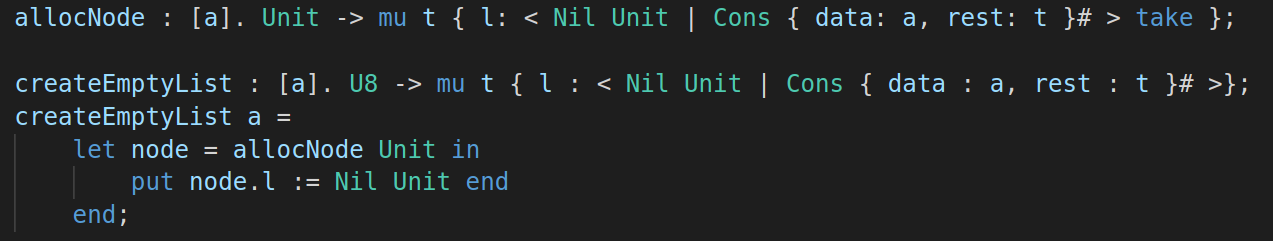
\includegraphics[width=\linewidth]{content/test1.png}
    \caption{Testing the construction of an empty list \todo{Replace images with LaTeX'd code?}}
    \label{fig:test1}
\end{figure}

These tests also test the intended effects of our new types, such as the strict positivity guarantee they provide
and their interaction with the existing type system. Whilst the existing tests test the backwards compatability of
record types, our new tests check that no recursive parameters are used non-strictly positive, that shadowing of recursive
parameters behaves as intended, and that recursive parameters are seperate from quantified type variables.

\autoref{fig:test2} shows a function with a non-strictly positive occurence of a recursive parameter nested in 
a negative position as the return type of a a function that is an argument. This program is rejected by the reorganiser
as shown in \autoref{fig:test2result}, which shows the recursive parameter $t$ that occurrs non-strictly positive.

\begin{figure}
    \centering
    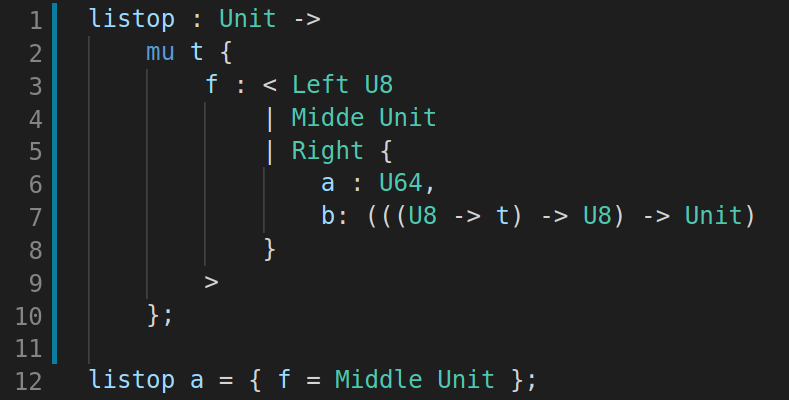
\includegraphics[width=0.8\linewidth]{content/test2.png}
    \caption{A non-strictly positive function}
    \label{fig:test2}
\end{figure}

\begin{figure}
    \centering
    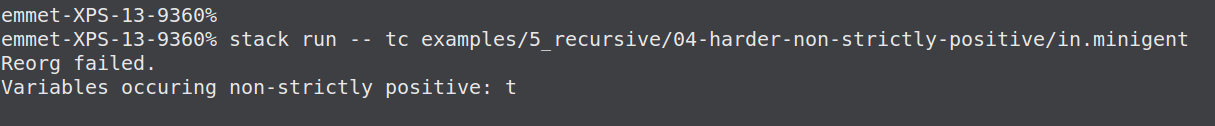
\includegraphics[width=\linewidth]{content/test2result.png}
    \caption{Running the Minigent typechecker on the program in \autoref{fig:test2}}
    \label{fig:test2result}
\end{figure}

\section{Potential Extensions}
\label{sec:proposedextensions}

This project allows for multiple potential extensions after the initial core development has been completed.
Some potential extensions if time allows are:

\begin{itemize}
    \item Adding a check that functions are primitive recursive within minigent, introduce a new keyword
          to require that a function is primitive recursive in minigent (i.e. the same as
          Isabelle's \textbf{primrec}).
    \item Write a small standard library of recursive data types, e.g. lists, binary trees, 
          sets.
\end{itemize}